% This Source Code Form is subject to the terms of the Mozilla Public
% License, v. 2.0. If a copy of the MPL was not distributed with this
% file, You can obtain one at https://mozilla.org/MPL/2.0/.

\documentclass[a4paper, 12pt]{article}

\usepackage[english, russian]{babel}
\usepackage[T2A]{fontenc}
\usepackage[utf8]{inputenc}
\setlength{\parindent}{1cm}
\usepackage{graphicx}
\usepackage{amsmath}

\begin{document}
	\begin{center}
		\section*{Расчётное задание по теоритической механике: кинематика твёрдого тела}
		\subsubsection*{Студент второго курса Физико-механического интститута, высшей школы МПУ: Куликовских Илья Михайлович}
		\subsubsection*{группа: 5031503/30001}
		\subsubsection*{Преподаватель: Аюпова Галина Константиновна}
	\end{center}
	$ $
	\textbf{Задача 1.} При поднятии ведра из колодца ускорение ворота диаметром  2.2, см, на который наматывается цепь, изменяется согласно графику на рисунке.
	Определить наибольшую скорость подъема ведра и высоту подъема за
	20 секунд.
	
	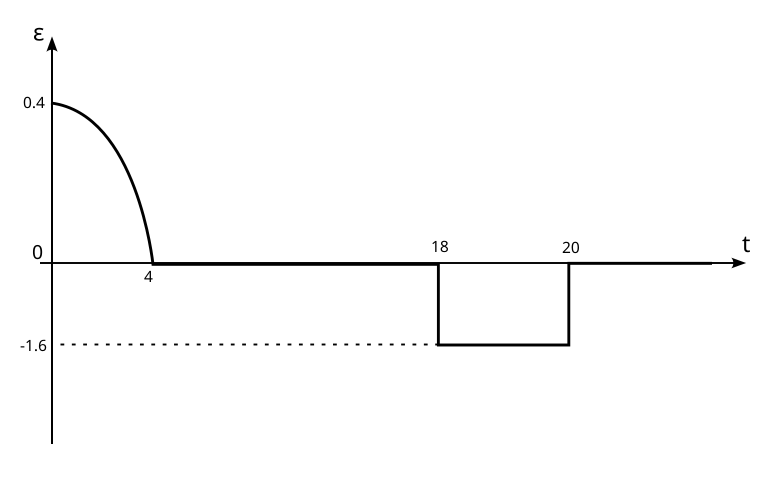
\includegraphics[width=0.8\textwidth]{screenshot001.png}
	
	\textbf{Решение: } Определим фунцию $\varepsilon$(t) как кусочно заданую, состоящую из параболы и двух линейных участков. Таким образом получившаяся функция имеет вид:
	
	\begin{center}
		$\varepsilon$(t) = 
		$\begin{cases}
			 -0.025t^2 + 0.4, t \in [0,4] \\
			 -1.6, t \in [18, 20] \\
			 0, t \in (4, 18) \cap (20, + \infty ) \\
		\end{cases}$
	\end{center}
	
	Знает каждый инженер: $\upsilon$ = $\omega$R, а значит для нахождения скорости достаточно найти интеграл $\int\varepsilon(t)dt$ и умножить на радиус.
	\begin{center}
		$\omega = \int\varepsilon(t)dt = \int(-0.025t^2 + 0.4)dt = -\frac{0.025}{3}t^3 + 0.4t + C$
		
		Н.у.: $\omega = 0$ если t=0, следовательно: C = 0
		
	\end{center}
	
	
	
\end{document}